\documentclass[a4paper]{article}

\usepackage[francais,english]{babel}
\usepackage[T1]{fontenc}
\usepackage[]{fullpage}
\usepackage{graphicx}
\usepackage{hyperref}
\usepackage[utf8]{inputenc}
\usepackage{subfigure}

\makeatletter
\def\thickhrulefill{\leavevmode \leaders \hrule height 1pt\hfill \kern \z@}
\def\maketitle{%
  \null
  \thispagestyle{empty}%
  \vskip 1cm
  \begin{flushright}
        \normalfont\Large\@author
  \end{flushright}
  \vfil
  \hrule height 2pt
  \par
  \begin{center}
        \huge \strut \@title \par
  \end{center}
  \hrule height 2pt
  \par
  \vfil
  \vfil
  \null
\begin{center}
\Huge{Placement constraints for a better QoS in clouds}
\end{center}
\begin{figure}[!ht]
	\centering
	\includegraphics[scale=.45]{imgs/cloud.png}
\end{figure}
\vfil
\begin{figure}[!ht]
	\centering
	\includegraphics[scale=.5]{imgs/polytech.png}
\end{figure}
\vfil
\begin{description}
	\item[Entreprise] Université de Nice-Sophia Antipolis
	\item[Lieu] Sophia-Antipolis, France
	\item[Responsable] Fabien Hermenier, équipe OASIS,
		\href{mailto:fabien.hermenier@unice.fr}{fabien.hermenier@unice.fr}
\end{description}
\cleardoublepage
}
\makeatother
\author{Mathieu Bivert, CSSR, \href{mailto:bivert@essi.fr}{bivert@essi.fr}}
\title{PFE: Cahier des charges (DOW)}

\begin{document}
\maketitle

\selectlanguage{francais}
\begin{abstract}
Dans le cadre de la répartition de machines virtuelles sur un ensemble de
serveurs physiques, ce projet vise à formaliser puis implémenter des
contraintes de placement, portant sur le type de systèmes de virtualisation.
Avant de s'intéresser à ces contraintes, il est nécessaire de doter BtrPlace
d'un tel système de typage.
\end{abstract}

\selectlanguage{english}
\begin{abstract}
Within the framework of placing virtual machines on a set of physical servers,
this project aims to formalize and to implement placement constraints,
relative to the type of different virtualization systems. Before thinking
about those constraints, BtrPlace needs to be extended in order to support such
a type system.
\end{abstract}

\tableofcontents
\newpage
\section{Description du projet}
\subsection{Contexte de travail}
Le monde industriel étant de plus en plus informatisé, la qualité des
réseaux s'améliorant, les sociétés informatiques tendent à  louer des
structures informatiques accessibles à distance.

Une société spécialisée dans l'automobile par exemple, a tout intérêt
à déporter la charge de conception et de maintenance de ses systèmes
d'informations à un hébergeur de services, spécialisée dans ce domaine.
En raison d'une plus grande expertise, cette dernière sera en effet beaucoup
plus performante, engendrant alors une baisse des coûts pour l'entreprise
cliente.

On notera cependant que toutes les entreprises n'ont pas forcément
interêt à exporter leur centre de traitement de l'information : par
exemple des structures reposant sur des données hautement confidentielles,
comme la recherche de pointe, l'armée ou les états.

Le terme de \og cloud \fg\ correspond à un certain nombre de serveurs
physiques et de logiciels, utilisés par une entreprise de services. Ces
dernières se déclinent en plusieurs types selon le(s) service(s) qu'elles
proposent, par exemple:
\begin{center}
\begin{tabular}{c|c|c|c}
	\textbf{Acronyme} & \textbf{Service} \textbf{fourni} & \textbf{Description} & \textbf{Exemple} \\
	\hline
	\hline
	SaaS & Software & Accès à un logiciel &
		Gmail\footnote{\url{https://gmail.com}} \\
	\hline
	PaaS & Platform & Une pile logicielle pour le développement &
		Google Apps\footnote{\url{https://www.google.com/enterprise/apps/business/}} \\
	\hline
	IaaS & Infrastructure & Accès à des ressources matérielles &
		Amazon EC2\footnote{\url{https://aws.amazon.com/ec2/}} \\
	\hline
	DaaS & Data & Accès à des données &
		Dropbox\footnote{\url{https://www.dropbox.com/}}
\end{tabular}
\end{center}

En particulier, un cloud \textit{IAAS} fournit à l'utilisateur un accès
à un ensemble de systèmes d'exploitations. Ces derniers sont très
souvent virtualisés, ce qui présente l'avantage de pouvoir faire tourner
plusieurs OS sur un même serveur physique. La virtualisation repose sur
un \textit{hyperviseur}, c'est-à-dire un moniteur de machines virtuelles (VM), dont
le but est de réaliser l'isolation entre les différentes VMs ainsi que de les administrer.
Cette tâche d'administration consiste essentiellement à démarrer, arrêter, migrer,
régler les ressources desdites VMs.

Par exemple, la figure \ref{hubertfxen} montre l'hyperviseur \textit{Xen}~\cite{barham2003xen}
sous NetBSD en train de virtualiser un FreeBSD, deux NetBSDs et une Debian.
\begin{figure}[!ht]
	\centering
	\includegraphics[scale=.17]{imgs/hubertf-xen.png}
	\caption{\label{hubertfxen} Virtualisation avec Xen; trois clients
		VNC \protect\footnotemark sont lancés pour accéder aux VMs}
\end{figure}

Une problématique pour les gestionnaires d'IAAS est donc de pouvoir placer
correctement un ensemble de VMs sur un ensemble de serveurs physiques.
Ce placement n'est pas libre : il est régit par un ensemble de contraintes,
éventuellement variables, devant être satisfaites.

\subsection{Motivations}
La virtualisation présente plusieurs avantages:
\begin{itemize}
	\item sur une application dite $n$-tiers, il est possible
	de placer chaque tiers sur une VM, et éventuellement d'en faire
	des duplications, ce qui améliore la robustesse de l'application.
	Par exemple, en cas de défaillance d'un serveur physique, il est
	stratégique d'avoir placé le réplicat d'un serveur de base de
	données sur un serveur différent de l'original;
	\item l'admninistration et la gestion des machines est simplifiée :
	il y a moins de hardware, donc moins de maintenance physique;
	la possibilité de pouvoir cloner, charger, décharger à la volée des
	VMs permet d'améliorer la QoS. Notamment, dans le cas
	où l'administrateur doit effectuer une opération de maintenance sur
	un serveur physique, il va devoir migrer~\cite{clark2005live} les VMs
	sur un autre serveur;
	\item chaque application peut être répartie sur une VM différente.
	Ainsi, si une application est compromise, elle a moins de chances
	de pouvoir compromettre d'autres applications que si elles étaient
	toutes lancées sous un même OS;
	\item utilisation plus performante du matériel, lorsqu'un ordinateur
	puissant peut être utilisé au maximum de ses performances en faisant
	tourner plusieurs systèmes d'exploitations. Cependant, utiliser un
	serveur à $99\%$ de ses capacités n'est pas toujours judicieux, puisque celui-ci
	sera alors incapable d'assurer une augmentation de charge. Il est donc
	impératif d'éviter une saturation;
	\item $\ldots$
\end{itemize}

% for hubertfxen; can't be in \caption; may need te be moved later to
% appears on the same page than the graphics
\footnotetext{\url{http://www.hep.phy.cam.ac.uk/vncdocs/index.html}}

La question de la répartition des machines virtuelles sur les machines
physiques se pose alors pour des raisons diverses et variées:
\begin{description}
	\item[maintenance] un serveur physique peut tomber en panne, ou
		nécessiter une réparation, auquel cas les programmes
		tournant dessus doivent être migré ailleurs, afin de
		garantir au client la qualité de service (QoS) qui lui est due;
	\item[sécurité] il peut s'avérer risquer pour un programme d'un
		client traitant des données sensibles (eg. données bancaires)
		de se retrouver au même endroit qu'un programme d'un
		autre client;
	\item[évolution des besoins] où au cours d'un certain intervalle de
		temps, les besoins en puissance de calcul d'une entreprise
		peuvent croître (suite à une plus grande popularité par
		exemple), ou encore la charge pouvant augmenter de façon
		brusque, voire irrégulière, aux heures de pointe;
	\item[économie d'énergie] où il peut être avantageux de réduire
		le nombre de serveurs physiques allumés, pour maximiser
		le rendement des autres machines physiques du cloud;
	\item[QoS] où, à l'inverse de l'économie d'énergie, il est bon
		de garder des ressources supplémentaires disponibles immédiatement,
		de façon à ne pas perdre de temps (et donc en QoS) à redémarrer
		un autre serveur;		
	\item[licence] les entreprises fournissant les systèmes de virtualisation
		proposent des licences selon différents critères, comme le nombre de
		machines virtuelles lancées, ou l'utilisation de ressources (CPU, RAM et bande passante
		principalement);
	\item[plateforme] plusieurs plateformes de virtualisations sont disponibles
		(eg. Xen, VMWare, Citrix); comme à un instant donné un serveur physique
		ne peut faire tourner qu'un seul type de plateforme, une nouvelle contrainte
		sur la répartition des machines virtuelles se pose.
	\item[] $\ldots$
\end{description}

Enfin, on notera que ces besoins fluctuent au cours du temps; les systèmes
de placement doivent donc être flexibles, au moins à deux niveaux.
D'abords, ils doivent être \textit{configurables}, afin de prendre en compte
les spécificités et les propriétés, éventuellement variables, des applications
et du datacenter. Une deuxième propriété d'\textit{extensibilité} est nécessaire,
pour être capable de supporter de nouvelles fonctionnalités au fur et à mesure
de l'évolution des besoins.

\subsection{Défis}
Cette extensibilité passe par un ajout aussi aisé que possible de nouvelles
contraintes. Le contexte fortement combinatoire (eg. le placement d'une VM
influe sur celui des autres) rend cette tâche difficle.

BtrPlace~\cite{herm2012} est un algorithme de placement de machines virtuelles,
implémenté dans le manager de clusters Entropy~\cite{herm2009}. Il utilise la programmation par
contraintes~\cite{rossi-handbook} à travers la bibliothéque Java Choco~\cite{choco}
pour trouver une solution au placement. L'ajout de nouvelles contraintes en quelques dizaines
de lignes de code sous forme de plugins garanti le besoin d'extensibilité précédemment
formulé. Enfin, par rapport aux autres avancées dans ce domaine, BtrPlace trouve
des solutions de placement assez rapidement, par exemple $3$ minutes pour $5000$
serveurs et $30000$ VMs.

\subsection{Objectifs}
Actuellement, plusieurs des points besoins cités au niveau de la répartitions des
VMs ne sont pas forcément implémentés ou formalisés entièrement. Le projet consiste
à choisir l'un de ces domaines et à l'ammener vers une forme satisfaisante.

Le dernier point est celui sur lequel porte ce projet, à savoir rendre BtrPlace
capable de gérer plusieurs types de VMs. Le travail sera
d'autant plus original que les questions d'économies d'énérgies sont historiquement
très prisées par les chercheurs, au détriment des autres.

Au sein d'une infrastructure, plusieurs types d'hyperviseurs, et donc de VMs, doivent
être supportés. Afin de satisfaire le critère de flexibilité, on peut avoir
besoin de changer le système de supervision des VMs d'un serveur à la volée.
Par exemple, on peut désirer vouloir garantir une certaine proportion
d'une plateforme donnée, un nombre maximum de VMs d'un certain type.

De ce point de vue, BtrPlace est incomplet : il ne permet pas de gérer le type
des VMs/plateformes, ni les étapes de reconfiguration nécessaires à un changement
d'hyperviseur. Dans ce sujet, on étendra donc dans un premier temps le modèle actuel
pour supporter le typage des infrastructures. C'est-à-dire, fournir
une implémentation de base permettant d'associer un type à une machine
virtuelle, et un ensemble de types possibles pour un serveur. En effet,
ces derniers peuvent ne pas supporter n'importe quel hyperviseur.

Dans un second temps, on modélisera et implémentera un ensemble de contraintes
pour contrôler les plateformes selon leur type. Par exemple, on peut limiter le
nombre de plateformes d'un type donné ou encore interdire un changement de type
sur un serveur.

\subsection{Scénario}
\begin{figure}[!ht]
	\centering
	\subfigure[Avant la reconfiguration] {
		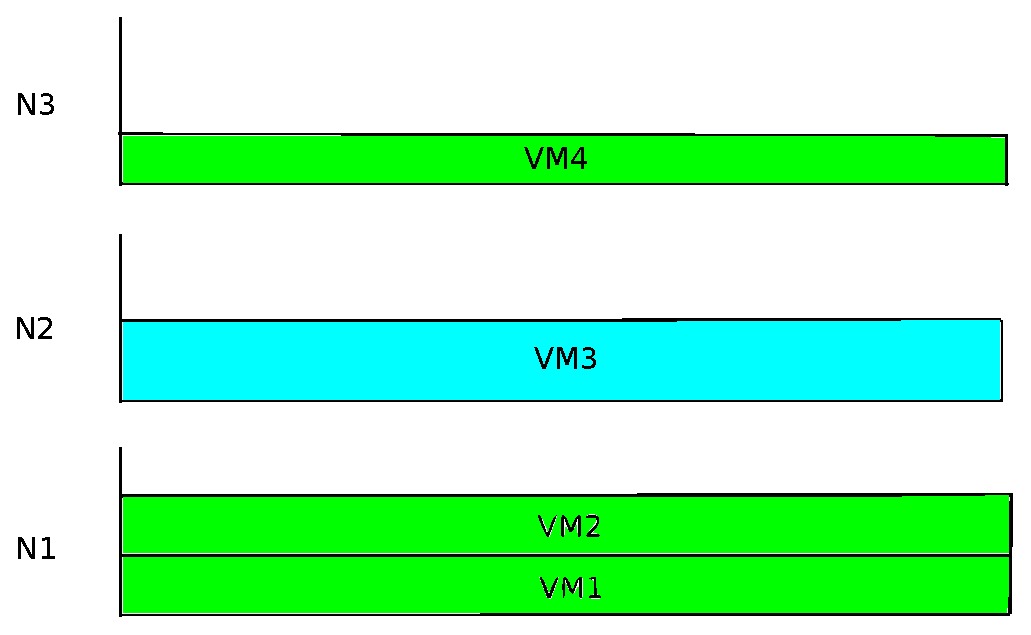
\includegraphics[scale=.40]{imgs/startreconf.eps}
		\label{startreconf}
	}
	\subfigure[Après la reconfiguration] {
		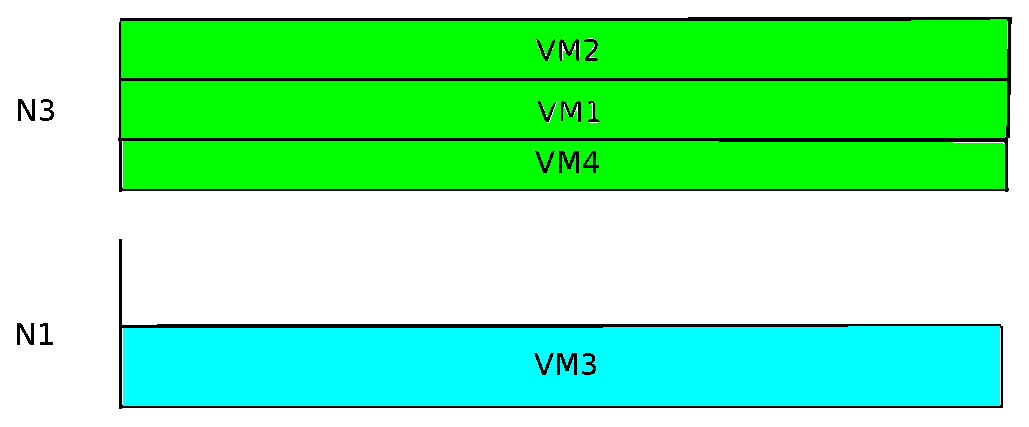
\includegraphics[scale=.40]{imgs/endreconf.eps}
		\label{endreconf}
	}
	\caption{\label{reconf} Exemple de changement de système de
		virtualisation. En vert des VMs Xen, en cyan une VM VMWare}
\end{figure}

Sur le diagramme \ref{startreconf}, on souhait mettre le serveur physique
$N_2$ hors-ligne pour des questions de maintenance. On utilise pour cela
la contrainte \textit{offline($N_i$);}\footnote{\url{http://www-sop.inria.fr/members/Fabien.Hermenier/btrpcc/offline.html}}.

Comme aucun serveur VMWare n'est disponible, il est nécessaire de supprimer
un serveur Xen, capable d'accueillir $VM_3$, par exemple $N_1$. Les machines
virtuelles situées sur ce dernier, $VM_1$ et $VM_2$,  doivent dans un premier
temps être migrées sur un autre serveur.

Puis, $N_1$ doit s'éteindre et redémarrer en changeant son système
de virtualisation. Enfin, la $VM_3$ est déplacée sur $N_1$, et $N_2$ peut
être éteint. L'état final est décrit par le diagramme \ref{endreconf}.

\subsection{Critère de succès}
L'extension apportée à BtrPlace devra supporter correctement les problèmes
de dépendances sur le placement des VMs, le typage des serveurs et les éventuels
changement dynamique de type de ceux-ci. Enfin, les contraintes doivent être
censées, bien définies, et répondre à des besoins concrets.

\section{État de l'art}
\subsection{Description générale}
Historiquement, les gestionnaires de placement se sont concentrés sur
le placement des VMs selon leurs besoins en ressources (CPU, RAM, BP, etc.),
tout en cherchant à réduire la consommation énergétique

Traditionnellement, ces approches reposent sur des algorithmes ad'hoc, rapides,
pour répartir les VMs. D'autres algorithmes plus flexibles ont vu le jour
suite aux demandes des clients, par exemple portant sur la fiabilité des
applications.

L'approche prise par \cite{jung2010} consiste à utiliser une fonction
d'utilité pour les applications à haute disponibilité. Leur solution
est prévue pour fonctionner dans le cas d'une défaillance d'un serveur
physique, mais n'est nullement adaptée pour répondre à des changements
de charge. De plus, l'ajout de nouveaux paramètres tels que la gestion
des types des serveurs nécessite de revoir l'algorithme de reconfiguration.
Enfin, les tests sont limités à un datacenter d'une douzaine de serveurs.

VMWare DRS~\cite{DRS} suit une approche similaire à celle de BtrPlace, en donnant
à l'administrateur un accès à quelques contraintes (plus ou moins
équivalentes à \textit{ban}, \textit{fence}, \textit{gather} et \textit{spread}).
Cependant, leur version de \textit{spread} ne garantit pas que lors
du déplacement d'une VM, l'ancienne et la nouvelle version de celle-ci
ne vont pas se superposer. DRS n'est pas prévu pour être étendu, et
il lui manque $5$ contraintes par rapport à BtrPlace. Enfin, l'administration
est limitée à des clusters de $32$ serveurs.

Entropy est à l'origine de BtrPlace. La programmation par contraintes
est utilisée pour placer les VMs sur un nombre minimum de serveur.
L'ordonnancement des actions nécessaires à la migration étant calculé
avec une heuristique ad'hoc, il est impossible d'ajouter des
contraintes telles que \textit{spread}, qui affectent l'ordonnancement.
Finalement, l'algorithme prend en compte toutes les VMs en marche lorsqu'il
cherche à résoudre un mauvaise placement, ce qui en pratique limite le nombre
de serveurs gérés à quelques centaines.

Récemment, de nouvelles approches plus flexibles ont vu le jour;
elles permettent d'intégrer des contraintes de placement à la
demande. Bin et al. utilisent aussi la programmation par contraintes
pour fournir un gestionnaire de placement modulaire. Ils
permettent une haute-disponibilité en garantissant qu'à chaque instant,
un certain nombre de serveurs sera disponible pour satisfaire
la consommation de ressources des VMs, et les contraintes de
déplacement. Lorsqu'un serveur a de fortes chances de tomber en panne,
les VMs sont migrées sur un autre, capable de satisfaire leurs besoins. Le modèle
proposé ne supporte pas les contraintes portant sur la gestion de
l'état des serveurs, l'ordonnancement des actions, ou encore sur la
façon dont les VMs sont migrées. Enfin, l'extensibilité n'a été
vérifiée que pour $32$ serveurs physiques et $128$ VMs au maximum.

Quelques aspects théoriques de BtrPlace ont été étudiés au préalable,
avec un premier prototype prenant en compte les ressources allouées
aux VMs, leur placement et l'étape de migration. \cite{herm2012}
étends ce travail en montrant que BtrPlace est capable de gérer
des datacenters de plusieurs centaines de serveurs. BtrPlace
est donc à l'heure actuelle le gestionnaire le plus efficace en
ce qui concerne le placement de VMs, tout en rendant possible
le contrôle de l'état des serveurs et les sur-allocations de ressources.
L'addition d'une dizaine de nouvelles contraintes répondant à
ces besoins démontre une extensibilité correcte. L'utilisation
d'une heuristique basée sur une optimisation de filtre
rends BtrPlace jusqu'à $20$ fois plus rapide sur la gestion de
datacenters composés de $2500$ serveurs.

Enfin, plusieurs plateformes expérimentales permettent de changer
l'OS tournant sur un nœud. Grid'5000~\cite{g5k}, reposant sur
Kadeploy\footnote{\url{http://kadeploy.imag.fr/}}, un ensemble
d'outils permettant de manager un ensemble de nœuds, utilise
OAR, un algorithe de réservations de ressources. Une autre
plateforme, Emulab~\cite{emulab} utilise Assign~\cite{ricci2003solver}
comme algorithme de placement.

Aucun des deux algorithmes utilisés par ces plateformes
ne supporte des contraintes,la gestion de licence, ou encore la
préparation de plateforme à l'avance.

Donc pour résumer, aucun système existant hormis BtrPlace ne passe
à l'échelle correctement, et aucun ne supporte le typage des VMs/nœuds,
ni même les moyens de l'exprimer telle quelle avec leur modèle.

\section{Méthodologie et planification}
\subsection{Stratégie générale}
La nature même du projet induit une stratégie \og linéaire \fg. L'étude
bibliographique pourra être étendue sur tout le projet en fonction
des besoins. Il en est de même pour la rédaction du rapport final, mais
pour d'autres raisons : il pourra servir de carnet de bord, ce
statut garantissant sa complétude vis-à-vis du travail fourni.

\subsection{Découpage en lots}
% \begin{enumerate}
% 	\item management du projet;
% 	\item étude bibliographique;
% 	\item rédaction du cahier des charges;
% 	\item extension de BtrPlace pour le support du typage;
% 	\item formalisation de contraintes utilisant l'extension précèdente;
% 	\item implémentation de ces contraintes;
% 	\item rédaction du rapport;
% 	\item création du support de présentation.
% \end{enumerate}
\begin{center}
\begin{tabular}{c|c|c|c|c|c}
	Id & Titre du lot & Type & Budget & Début (inclus) & Fin (inclus) \\
	\hline
	\hline
	$L_1$ & Management du projet & MGMT & $38$ & $S_3$ & $S_{20}$ \\
	\hline
	$T_{1.1}$ & Planification & MGMT & $19$ & $S_3$ & $S_{20}$ \\
	\hline
	$T_{1.2}$ & Suivi du projet & MGMT & $19$ & $S_3$ & $S_{20}$ \\
	\hline
	$L_2$ & Étude bibliographique & RECH & $38$ & $S_3$ & $S_5$ \\
	\hline
	$L_3$ & Cahier des charges & REDAC & $38$ & $S_3$ & $S_4$ \\
	\hline
	$L_4$ & Extension pour le typage & IMPL & $38$ & $S_6$ & $S_{12}$ \\
	\hline
	$L_5$ & Ensemble de contraintes & RECH/IMPL & $38$ & $S_{13}$ & $S_{14}$ \\
	\hline
	$T_{5.1}$ & Formalisation des contraintes & RECH & $19$ & $S_{13}$ & $S_{14}$ \\
	\hline
	$T_{5.2}$ & Implémentation des contraintes & IMPL & $19$ & $S_{15}$ & $S_{17}$ \\
	\hline
	$L_6$ & Rédaction du rapport & REDAC & $38$ & $S_3$ & $S_{20}$ \\
	\hline
	$L_7$ & Création du support de présentation & DEMO & $38$ & $S_{19}$ & $S_{20}$ \\
\end{tabular}
\end{center}
\subsection{Plannification}
gantt redondant avec le découpage en lots tel que spécifié.
\subsection{Livrables associés au projet}
\begin{center}
\begin{tabular}{c|c|c|c|c}
	Id & Titre du livrable & Lot(s) & Nature & Date \\
	\hline
	\hline
	$D_1$ & Cahier des charges & $1$ & Document & $S_4$ \\
	\hline
	$D_2$ & Gestion du typage et du déploiement & $1$ & Document & $?$ \\
	\hline
	$D_3$ & Ensemble de contraintes & $1$ & Document et Logiciel & $?$ \\
	\hline
	$D_4$ & Rapport de management & $1$ & Document & $S_{20}$ \\
	\hline
	$D_5$ & Diaporama de présentation & $1$ & Document & $S_{20}$ \\
\end{tabular}
\end{center}

\subsection{Jalons}
\begin{center}
\begin{tabular}{c|c|c|c|c}
	Id & Jalon de fin de phase & Lot(s) & Date & Vérification \\
	\hline
	\hline
	$J_0$ & planification & $1$ & $S_4$ & $D_1$ \\
	\hline
	$J_1$ & formalisation & $1$ & $S_n$ & $D_2$ partiel \\
	\hline
	$J_2$ & implémentation & $1$ & $S_{n+k}$ & $D_3$, $D_2$ partiel \\
	\hline
	$J_3$ & projet & $1$ & $S_{20}$ & $D_2$, $D_3$, $D_4$ et $D_5$ \\
\end{tabular}
\end{center}

\subsection{Pilotage et suivi}
Une réunion à l'INRIA avec l'encadrant par semaine au minimum, pour
constater le bon avancement du projet, plus si besoin. Contacts par
email plusieurs fois par semaine.

\section{Description de la mise en œuvre du projet}
\subsection{Interdépendance des lots et tâches}
Pour les deux lots composés $L_1$ et $L_5$:
\begin{figure}[!ht]
	\centering
	\subfigure[$L_1$] {
		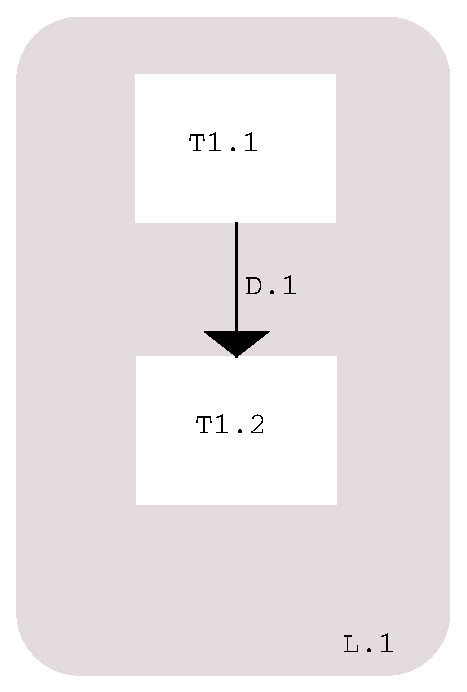
\includegraphics[scale=.45]{imgs/L1.eps}
	}
	\subfigure[$L_5$] {
		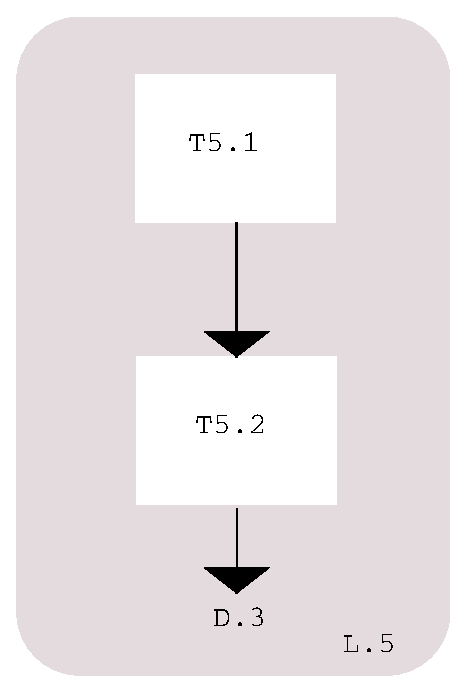
\includegraphics[scale=.45]{imgs/L5.eps}
	}
%	\caption{\label{lotscomp} Lots $L_1$ et $L_5$}
\end{figure}

Pour les autres, en raison de leur extrème simplicité, on se contente d'une
description textuelle:
\begin{itemize}
	\item Les lots \og Cahier des charges \fg\ et \og Étude bibliographique \fg\
		sont des prérequis au livrable \og cahier des charges \fg\ ($L_2, L_3
		\Rightarrow D_1$);
	\item le lot d'\og Extension de typage \fg\ est un prérequis au livrable
		\og Gestion du typage et déploiement \fg\ ($L_4 \Rightarrow D_2$);
	\item le lot d'\og Rédaction du rapport \fg\ est un prérequis au livrable
		\og Rapport de management \fg\ ($L_6 \Rightarrow D_4$);
	\item le lot d'\og Création du support \fg\ est un prérequis au livrable
		\og Diaporama de présentation \fg\ ($L_7 \Rightarrow D_5$);
\end{itemize}
Enfin, comme mentionné à plusieurs reprises auparavant, les contraintes ne peuvent
être implémentées sans un système de typage fonctionnel dans BtrPlace.
\subsection{Description des lots}
\subsection{Résumé de l'effort}
\subsection{Gestion du risque}
En cas de blocage sur l'implémentation du typage, une réfléxion sur
les contraintes pourra toujours avoir lieu, mais ne déboucherait pas
sur une implémentation valide.
\section{Participants}
\subsection{Mathieu Bivert - CSSR}
Étudiant à Polytech'Nice Sophia, spécialisé en Cryptographie, Systèmes
Sécurité et Réseaux.

\subsection{Fabien Hermenier - OASIS/INRIA}
\textbf{Fabien Hermenier} a recu un doctorat en $2009$ à l'université
de Nantes. Depuis $2011$, il enseigne en tant que Maître de conférence
à l'université de Nice Sophia-Antipolis. Son travail de recherche
s'articule autour des plateformes d'hébergement, de la virtualisation,
du calcul autonome et de la gestion des ressources. Depuis $2006$, il
travaille sur des algorithmes de placement de machines virtuelles pour
faire face à l'augmentation des SLA dans les plateformes d'hébergements.

\newpage
\selectlanguage{francais}
\bibliographystyle{alpha}
\bibliography{docs}

\end{document}

